\documentclass[12pt]{extarticle}
\usepackage{algorithm}


\usepackage{amsmath}
\usepackage{algpseudocode}
\usepackage[%
    left=1.3in,%
    right=1.3in,%
    top=1.1in,%
    bottom=1.1in,%
    paperheight=11in,%
    paperwidth=8.5in%
]{geometry}%

\usepackage[english]{babel}
\usepackage{blindtext}
\usepackage[]{hyperref}
\hypersetup{colorlinks=false,linkcolor=false,pdfborder = {0 0 0}
}
\geometry{top=2cm,bottom=2cm}
\usepackage{setspace}
\usepackage{graphicx}
\graphicspath{{images/}}
\onehalfspacing

\usepackage{tabularx}
\usepackage{caption}
\usepackage{subcaption}
\usepackage{pdfpages}
\usepackage{afterpage}

\usepackage[acronym]{glossaries}
\newacronym{ny}{NY}{New York}
\begin{document}


\newpage
\pagebreak
\hspace{0pt}
\vfill
\begin{center}
\section{Résume}
\end{center}
\vfill
\hspace{0pt}
\pagebreak



La robotique en essaim est un domaine en pleine expansion qui consiste à coordonner des groupes importants de robots pour qu'ils coopèrent afin d'atteindre un objectif commun. Les robots en essaim tentent de résoudre de multiples tâches et problèmes, dont l'un est le problème de la formation de motifs, où les robots tentent de former des formes géométriques. Il y a de nombreuses applications dans l'agriculture, la recherche et le sauvetage, et les entrepôts. L'une des méthodes utilisées pour contrôler l'essaim est les algorithme d'apprentissage par renforcement profond. Dans notre projet, nous avons utilisé l'algorithme DDPG pour contrôler l'équipe de robots afin de former des motifs avec l'aide d'un robot central qui surveillera et guidera les robots vers leurs objectifs cibles en générant des 
coordonnée  relative à sa position. Notre algorithme a obtenu  une précision de 92\% lorsqu'il a été testé sur un ensemble aléatoire de formes lorsque le nombre de robots est de 3, 4 et 5, mais la précision tombe à 80\% lorsqu'il est testé sur un groupe de six robots. où un autre type d'algothime doit être appliqué, comme le madppg, pour gérer un grand nombre de robots.\\


\textbf{Mots Clés}: Swarm robotics, Reinforcement lerarning, DDPG,Ros,Pattern foramtion,Gazebo


\newpage
\pagebreak
\hspace{0pt}
\vfill
\begin{center}
\section{Abstarct}
\end{center}
\vfill
\hspace{0pt}
\pagebreak


Swarm robotics is a fast-expanding field that includes coordinating sizable groups of robots to cooperate in order to achieve a common objective. There are multiple tasks and problems that swarm robots try to solve; one of them is the pattern formation problem, where the robots try to form geometric shapes. It has many applications in agriculture, search and rescue, and warehouses. One of the methods used to control the swarm is deep reinforcement learning algothims.In our project, we used the ddpg RL algorithm to control the team of robots to form some patterns with the help of a central robot that will monitor and guide the robots towards their target goals by generating the shape relative to his position. Our algorithm gets an accuracy of 92\% when tested on a random set of shapes when the number of robots is 3, 4, or 5, but the accuracy drops to 80\% when tested on a group of six robots.\\

\textbf{Keywords}: Swarm robotics, Reinforcement lerarning, DDPG,Ros,Pattern foramtion,Gazebo

\newpage
\thispagestyle{empty}
{
\hypersetup{linkcolor=false}
\tableofcontents

}




\newpage
\listoffigures
\clearpage

\newpage
\section*{Acronyms}

\hspace{0.5cm} \textbf{RL}  Reinfocement Learning

\vspace{0.2cm}

\textbf{SR} Swarm Robotics

\vspace{0.2cm}
\textbf{ROS} Roboting Operating System.

\vspace{0.2cm}

\textbf{DQN} Deep Q Learning.

\vspace{0.2cm}

\textbf{DRL} Deep Reinfocement learning.

\vspace{0.2cm}



\textbf{DDPG} Deep Deterministic policy gradient.

\vspace{0.2cm}

\textbf{LDS} Laser Distance Sensor.

\vspace{0.2cm}

\textbf{IMU} Inertial Measurement Unit.

\vspace{0.2cm}



  








\newpage
\pagebreak
\hspace{0pt}
\vfill
\begin{center}
\section{Introduction}
\end{center}
\vfill
\hspace{0pt}
\pagebreak

\subsection{Introduction}
These days, mobile robots have taken place in many fields like industry automation, planetary exploration, entertainment, construction, etc. because of their ability to work in extreme environments with high precision and without fatigue\cite{rubio2019review}.Even so, a robot occasionally needs the support of other robots because it is impossible or difficult for them to perform some tasks on their own. For that reason, a new field has emerged to deal with these problems, swarm robotics.
Swarm robotics is a relatively new research topic that has gained more attention in the last few years. It is about studying how a large number of simple robots (a swarm) can collaborate and work together to achieve predefined objectives and tasks that are often difficult or impossible to do for a single robot. \cite{bayindir2016review}.
This field has mainly focused on a set of problems that a swarm of robots normally faces. The most common problems are: aggregation, dispersion, pattern formation, coordinated movement, hole avoidance, and foraging.
The problem that will be studied in this thesis is pattern formation. Where the agents (robots) try to form different geometric shapes like squares, triangles, and circles in order to perform a specific task like lifting something, encircling some target, or for rescue operations.

We can solve this problem using two different approaches. The first one is a completely centralized method where there is a central unit that controls the swarm in all its actions and has global state access. However, this can be easy and much simpler, but it is less robust if the central unit fails. The second approach is a distributed one, where each robot uses local communication and has access only to his local state, which is much more scalable and robust but more complex and requires more time. \cite{bayindir2007review}
Our primary objective in this thesis is to implement an RL algorithm in a system made up of a group of robots in order to form some specific geometric patterns. We will not use a completely centralized method where each robot will move autonomously, but a central robot is needed to monitor and coordinate the others. We will be using deep reinforcement learning algorithms to train the agents to achieve their task.

This thesis is organized as follows: In the first chapter, we will define swarm robotics, its domains, applications, and common problems it tries to solve.
In the second chapter, we will define reinforcement learning, the most commonly used algorithms in this domain and how they work, and finally, how different papers have applied these algorithms to learning to navigate autonomous robots.
\pagebreak The third chapter will discuss the problem formulation in reinforcement learning and how we have designed our solution.
The fourth chapter will be about the implementation of our solution in the Ros framework and the gazebo simulator and how we set up networking between the robots.
Finally, the fifth chapter is the result analysis of our experiments and cites the goals we have achieved and the problems that arise.

   


  
 
 




\newpage
\pagebreak
\hspace{0pt}
\vfill
\begin{center}
\section{Swarm Robotics}
\end{center}
\vfill
\hspace{0pt}
\pagebreak




                  
\subsection{Swarm Intelligence and Social animal inspiration}
Social animal and insect behavior in groups like bees dancing, wasps nest-building, ants' collaboration, bird flocking, and fish schooling has caught the attention of researchers for their ability to archive complex tasks and work in coordination, which demonstrate some form of swarm intelligence that researchers have taken inspiration from to design and implement swarm robotics systems. \cite{navarro2013introduction}
They also report that social insects were able to accomplish their goals, like searching for food, alerting the presence of an enemy, or collaborating to lift heavy objects, without having access to the global state or having a leader to guide them. They were only able to accomplish this by utilizing local interactions and communication, which spread to other members and prompted group-wide cooperation. \cite{navarro2013introduction}


\subsection{Swarm robotics and multi robot systems}
The early 1980s were when multi-robot systems first gained popularity. As the name suggests, multi-robot systems introduce the idea of teamwork in order to complete tasks that are challenging or impossible to complete alone by the robots. Seven topics of study have been identified in this field, which include: 
\begin{itemize} 
\item Biological Inspirations; 
\item Communication 
\item Localization, Mapping, and Exploration;
\item Object Transport and Manipulation; 
\item Motion Coordination; 
\item Reconfigurable Robots. 
\end{itemize}

 

\subsection{Swarm robotics}
Swarm robotics has no one definition because it is a rapidly developing area and new research is constantly being done in it. But we can take this definition from a cited paper. "Swarm robotics is the study of how a large number of relatively simple physically embodied agents can be designed such that a desired collective behavior emerges from the local interactions among agents and between the agents and the environment." \cite{csahin2005swarm}.\\
The main characters of swarm robots are:
 \begin{itemize} 
\item The robots in the swarm must be autonomous.
\item The number of robots in the swarm is large.
\item Homogeneity is required for robots. A small number is acceptable if not.
\item Robots must be incompetent with regard to the primary task they must complete, otherwise, they will fail or perform poorly.
\item Robots are limited to local communication and sensing. It makes sure that coordination is spread, making scalability one of the system's characteristics. \cite{navarro2013introduction} \end{itemize}

\subsection{Swarm robotics properties}
Swarm robotics have some properties that describe the system's current condition. Below are some of these properties:

\textbf{Robustness}: The capacity of the swarm to continue operating even if certain group members die or some system components fail.\\ \textbf{Scalability}: The system's capacity to function successfully in both small and large group sizes without affecting the swarm's performance.

\textbf{Flexibility} The swarm's capacity to govern and adapt to environmental changes 

\textbf{Autonomus}: implies that there is no central authority controlling the behavior of the swarm and that each individual is independent of the others.

\textbf{Local communication} The communication among swarm members is local since they don't have access to the swarm's overall state. \cite{brambilla2013swarm}\cite{olaronke2020systematic}
  

\subsection{Domain of application}
In this section, we will list some of the significant domains where swarm robotics fits in and can impact solving the domain problem.\newpage
\subsubsection{Tasks that cover a region}
Swarm robots are best suited for handling issues that encompass an area of space because of the swarm's extensive sensing capabilities, such as monitoring the environment of a lake or surveillance of a particular region. \cite{csahin2005swarm}\cite{olaronke2020systematic}

\subsubsection{Search and rescue missions}
Swarm robots can be used for these sorts of tasks in various accidents or catastrophes, such as earthquakes, when human involvement is challenging. These robots include the M-TRAN, Polyobot, and Swarm Bot.

\subsubsection{Cleaning of oil speals}
Such problems may be handled more quickly and affordably with a swarm of robots. Seaswarm, a robot created by the senseable team at MIT, is an example of one used for such activities.

\subsubsection{Exploration}
To investigate Mars, swarm robots like Marsbees have been created. The same holds true for the CoCoRo swarm, which was employed for an in-depth underwater investigation.
\subsubsection{Agriculture}
As they are  used to enhance agriculture and keep an eye on the health of crops. 

\subsection{Swarm robotics basic tasks and problems}
SR tasks may be reduced to simple operations that the swarm often performs in an effort to achieve its goal.
Aggregation, dispersion, pattern development, coordinated movement, hole avoidance, and foraging are among these activities.\cite{bayindir2007review}\cite{navarro2013introduction}.

\subsubsection{Aggregation}
The robots are combined in order to complete a task or share information. In a centralized system, this task could be simple, but in a decentralized one, it might be challenging.
\subsubsection{Dispersion}
Sometimes, in order to increase the group's sensing capacities during exploration, the swarm must span a large region without losing contact with its members. 
\subsubsection{Pattern formation}
In order to carry things or navigate hallways, the swarm must sometimes create precise patterns such as circles, squares, or lines.
\subsubsection{Cordinated movement}
It is making an effort to coordinate the group movements by maintaining the established pattern between the robots.
\subsubsection{Hole avoidance}
As suggested by the name, the group makes an effort to avoid stepping into holes.
\subsubsection{Foraging}
The swarm aims to locate objects, pick them up, and position them where needed.





\begin{figure}
\centering

\begin{subfigure}{.5\textwidth}
  \centering
  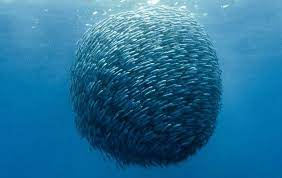
\includegraphics[width=.8\linewidth]{swarmfish}
  \caption{fish swarm }
  \label{fig:sub1}
\end{subfigure}%
\begin{subfigure}{.5\textwidth}
  \centering
  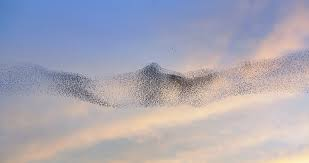
\includegraphics[width=.8\linewidth]{swarmbirds }
  \caption{birds swarm  }
  \label{fig:sub2}
\end{subfigure}
\caption{swarm animals}
\textbf{ref}:https://www.nationalgeographic.com/
\textbf{ref}:https://www.researchgate.net/
\label{fig:test}
\end{figure}



\subsection{Concultion}
In this section, we have defined swarm robotics, its properties and applications, and the problems or tasks that need to be solved by the team of robots. In the next chapter, we will introduce deep reinforcement learning and its applications in the swarm robotics field.


\newpage
\pagebreak
\hspace{0pt}
\vfill
\begin{center}
\section{Deep reinforcement learning}
\end{center}
\vfill
\hspace{0pt}

\pagebreak

\subsection{Introduction}
In this chapter, we will provide an overview of the field of reinforcement learning, including its applications, various techniques, and how it relates to swarm robotics. 
\subsection{Machine learning}
Machine learning is a subfield of artificial intelligence that focuses on developing algorithms and models that make predictions and take decisions without being explicitly programmed to do so based on the input data they receive. Generally speaking, there are three types of machine learning algorithms: supervised algorithms, which obtain labeled data and attempt to categorize or anticipate the unknown. Unsupervised learning algorithms, where the data is unlabeled and it is the job of the ML algorithms to extract hidden patterns in it. And finally, reinforcement learning algorithms, where the algorithm learns to make decisions based on trial and error and rewards by interacting with an environment,

\subsection{Reinforcement learning}
Reinforcement learning algorithms are based on an agent that interacts with and observes an environment in order to take actions that maximize the reward for a given task.
The goal of the agent is to learn an optimal policy ($\Pi$) that maps states to actions in order to get the best possible action to take in a given situation. This can be achieved by maximizing the expected reward that the agent receives from the environment for each step he takes. \cite{arulkumaran2017brief}

Formally, RL can be described as a Markov decision process (MPD) where the future state depends only on the current one. An MPD consists of:

\begin{itemize}
  \item  A set of states $S$
  \item  A set of actions $A$
  \item  A transition dynamics $\rho(S_{t+1}|a,S)$. which give the probability of being in state $S_{t+1}$ based on the current state $S$ and the performed action $A$.
  \item A reward function $R(S_{t},A_{t},S_{t+1})$ which outputs a scalar reward $r_{t} \subset R$. 
   \item A discount factor $\gamma \in [0,1]$ which  emphasis either  immediate or future rewards.
\end{itemize}

\newpage
From the above definition, the policy function $\Pi$ will map a given state to a probabilistic distribution over actions: $\Pi: S \longrightarrow \rho(A=a|S)$. The goal of the agent is to find the optimal policy $\Pi$ that maximizes the expected return. \\
\[ \Pi^{*} = argmax_{\Pi}  E[R|\pi] \]



If the MPD is episodic, then the agent will accumulate a set of rewards at the end of each episode, which is called a return:

\[ R= \sum_{t=0}^{T-1} \gamma^{t}r_{t+1} \]



Setting $\gamma<1$ will ensure the convergence of the return in the case of non-episodic MPDS.\cite{arulkumaran2017brief}.

\subsection{Q learning}
Q-learning is a type of model-free reinforcement learning algorithm based on the dynamic programming technique, where the agent tries to maximize its rewards by finding the optimal policy $\Pi$ in an iterative manner. In order to achieve this, the agent uses a type of equation called a value function that gives it the value or reward of being in a state $s$ and taking action according to its policy $\Pi$.


\[ V^{\Pi}(S)=E[r(s,a)+\gamma V^{\Pi}(s') ] \] 

In order to find the optimal value function, hence finding the optimal policy, the equation must satisfy the Bellman optimality condition, which states that: 

  
\[ V^{*}(S)=max_{a}E[r(s,a)+\gamma V^{*}(s') ] \] 

The same goes for the action-value function, which gives the return if the agent chooses the action $a$ and follows the optimal policy thereafter.

\[ Q^{*}(S,a)=E[r(s,a)+max_{a}\gamma Q^{*}(s',a) ] \]\cite{watkins1992q}.


\pagebreak

\subsection{Deep Q learning}
The problem with traditional Q-learning or Rl algorithms in general is their inability to work in high-dimensional input states where discritization and hand-crafted feature extraction are performed in order to work. For this, deep learning was combined with traditional Q-learning in order to overcome these challenges. \cite{mnih2013playing}
Deep Q learning was first introduced in an article by the Deepmind group, where it was tested in atari games in which the agent was given raw input images of the emulator, and it was the goal of the agents to win the games by using the Q learning algorithm.
Besides using the Bellman equation to converge and calculate the loss, an experience replay memory was used to store the experiences of the agents during the game and then sampled randomly to be fed to the neural network to learn and to break the correlation that appears when feeding them sequential data. \cite{mnih2013playing}  

\begin{algorithm}
\caption{Deep Q-learning with Experience Replay}\label{alg:cap}
\begin{algorithmic}
\State Initialize replay memory D to capacity N
\State Initialize action-value function Q with random weights
\For{\texttt{episode = 1, M}}
        \State \texttt{Initialise sequence s1 = \{x1\} and preprocessed sequenced $\phi_{1}$ = $\phi(s_{1})$  }
        \For{\texttt{t = 1, T}}
         \State With probability $\epsilon$ select a random action $a_{t}$
         \State otherwise select  $a_{t}$ = $max_{a} Q^{*}(\phi(s_{t},a;\theta) $ 
         \State Execute action $a_{t}$ in emulator and observe reward ${r_{t}}$ and image $x_{t+1}$
        \State Set $s_{t+1}$ = $s_{t}$ , $a_{t}$ , $x_{t+1}$ and preprocess  
        $\phi_{t+1}=\phi(s_{t+1})$
        \State Store transition $(\phi_{t} , a_{t} , r_{t} , \phi_{t+1} )$ in $D$
        \State Sample random
minibatch of transitions $(\phi_{t} , a_{t} , r_{t} , \phi_{t+1} )$ in $D$
        \State set  \begin{equation}
  y_{j}=\begin{cases}
    r_{j}, & \text{for terminal $\phi_{j+1} $}.\\
    r_{j}+\gamma max_{a}Q(\phi_{j+1},a';\theta) , & \text{for non-terminal $Q(\phi_{j+1})$}.
  \end{cases}
\end{equation}
        \State Perform a gradient descent step on $(y_{j} - Q(\phi_{j} , a_{j} ; \theta))$ 
        \EndFor 
\EndFor 


\end{algorithmic}
\end{algorithm}
 


\pagebreak

\subsection{Deep Deterministic policy gradient }
One of the downsides of DQN is that  he can  only work  in discrete action spaces. For this reason, tasks that require continuous control, such as the linear and rotational movements of robots, require discretization. In most cases, this can result in a large action space, which slows convergence and causes instability.
For this, there is another type of DRL algorithm named Deep Deterministic Policy Gradient, which is a policy-based actor-critic algorithm that takes the benefits of both methods (the policy-based method and the value-based method) and uses the actor-critic to reduce the bias (underfitting) that occurs.
DDPG is composed of two neural networks: the actor and the critic. The job of the actor is to select an action based on the input state. And it is the critic who will determine if that action is suitable or not by observing the rewards returned when taking that specific action in a specific state.
The critic network is learned using the Bellman equation, the same as q-learning.
The DDPG algorithm also uses a replay buffer to store agent experiences in order to sample from them later when training the network.
Like in Q-learning, to enable better exploration for the agent, noise is sampled from a process $\eta$ then added to the output of the actor network. It is common to use the Ornstein-Uhlenbeck process to generate temporally correlated values. \cite{lillicrap2015continuous}


 \begin{figure}[h] 
\centering
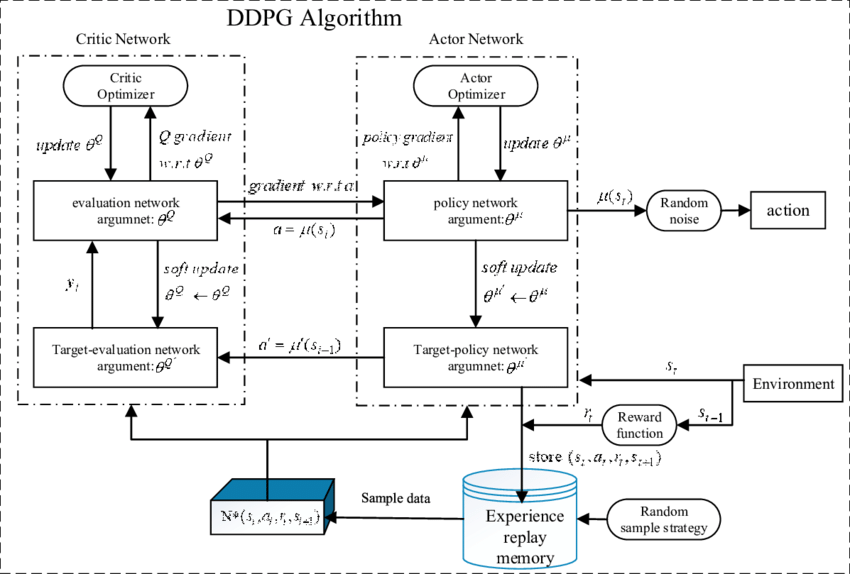
\includegraphics[scale=0.45]{ddpg}
\caption[ddpg]{ddpg \textbf{ref}:https://www.researchgate.net/]]}
\end{figure}



 
\begin{algorithm}[H]
\caption{Deep Deterministic Policy Gradient (DDPG)}
\label{alg:ddpg}
\begin{algorithmic}[1]
\State Initialize actor network $\mu(s|\theta^\mu)$ and critic network $Q(s,a|\theta^Q)$ with weights $\theta^\mu$ and $\theta^Q$
\State Initialize target networks $\mu'(s|\theta^{\mu'}) \leftarrow \mu(s|\theta^\mu)$ and $Q'(s,a|\theta^{Q'}) \leftarrow Q(s,a|\theta^Q)$ with weights $\theta^{\mu'} \leftarrow \theta^\mu$ and $\theta^{Q'} \leftarrow \theta^Q$
\State Initialize replay buffer $R$
\For{episode $=1$ to $M$}
\State Initialize a random process for action exploration
\State Receive initial observation state $s_1$
\For{$t = 1$ to $T$}
\State Select action $a_t = \mu(s_t|\theta^\mu) + \mathcal{N}t$ according to current policy and exploration noise $\mathcal{N}t$
\State Execute action $a_t$ and observe reward $r_t$ and new state $s{t+1}$
\State Store transition $(s_t, a_t, r_t, s{t+1})$ in $R$
\State Sample a random minibatch of $N$ transitions $(s_i, a_i, r_i, s_{i+1})$ from $R$
\State Set $y_i = r_i + \gamma Q'(s_{i+1},\mu'(s_{i+1}|\theta^{\mu'})|\theta^{Q'})$
\State Update critic by minimizing the loss: $\mathcal{L} = \frac{1}{N}\sum_i(y_i - Q(s_i,a_i|\theta^Q))^2$
\State Update actor policy using the sampled policy gradient: $\nabla_{\theta^\mu} J \approx \frac{1}{N}\sum_i \nabla_a Q(s,a|\theta^Q)|{s=s_i,a=\mu(s_i)} \nabla{\theta^\mu} \mu(s|\theta^\mu)|_{s_i}$
\State Update target networks: $\theta^{\mu'} \leftarrow \tau \theta^\mu + (1-\tau)\theta^{\mu'}$ and $\theta^{Q'} \leftarrow \tau \theta^Q + (1-\tau)\theta^{Q'}$
\EndFor
\EndFor
\end{algorithmic}
\end{algorithm}



\subsection{Related Work}
In this section, we present some of the work that has applied RL algorithms to training agents and robotic systems.

The most used algorithm is deep Q learning, where \cite{mnih2013playing} has applied  in learning to play atari games by using a convolutional neural network by providing raw image pixels as input, where they demonstrated that the agents achieved great performance, even surpassing human level.
In continuous action spaces, \cite{lillicrap2015continuous} have used the ddpg algorithm, which is an extension of the DQN and the DPG algorithms. They have used an actor-critic model-free policy-based algorithm that operates in contiguous action space by applying it to several simulated physics tasks, and also shows great results achieved by the agents.
in the field of multi-agents. \cite{diallo2020multi} where they used a decentrilized approach to train multi-agents to form some patterns using the DQN network with a central replay buffer that contains agents experiences in order for them to learn cooperatively.


in \cite{gong2022efficient} used the DDPG algorithm for path planning and control of a robot to reach its target position. Unlike traditional fully connected layers in the actor and critic layers of DDPG, they have fed the state of the robot to an LSTM layer, so the robot's decision is not based only on the current state but also the past state. The model was tested in different environments with and without obstacles and showed good results..

In \cite{prasad2017multi}, they used a decentrilized Deep Q network approach to train six robots to form polygon squares, where they set the target goals for the agents and designed a reward function to encourage them to reach their goals.



In \cite{long2018towards} have used the proximal policy optimization algorithm (PPO), which is a policy-based one, to control in a decentrilized manner a group of robots to reach their target by avoiding collisions between each other. To avoid collisions, they have used convultional neural networks to extract features from consecutive lidar measurements and then pass them through a dense layer with the robot's actions. The model was tested in different types of environments, and the robots were able to achieve their target goal successfully without collisions.

In \cite{diallo2020multi}, They used a multi-agent DQN algorithm to train agents to form some shapes based on local sensing. And to enable cooperation between the agents, they used a central replay memory to store their experiences instead of a local one. They also generated a random  set of shapes at the begining of each episode to avoid overfitting when testing.
The model was deployed, and the agents learned to form complex geometric shapes.


In \cite{ma2020multi} have used the DDPG algorithm to train multiple robots to encircle some target in a static position or in motion, where the agents (robots) learn to cooperatively accomplish their task by using a central replay memory. With robots having access to the target locations, they used a primary-based reward function to keep a distance and angle from it and from the neighboring robots. The models were deployed and tested to encircle static and moving targets, and they showed good results.


in \cite{bae2019multi}, a group of robots navigates an environment and moves in a predefined formation by working cooperatively. In this work, they combined CNN to analyze image data with Deep Q learning to train the robots to avoid each other and obstacles, then tested them in various environments, which showed good results.

Finnaly in \cite{wang2019pattern}, They used a novel approach to train multiple robots to form complex shapes. They split their work into two phases: training and execution. In the training phase, they used two networks, one for predicting actions and one for values, like the actor-critic method, but they used their own extended PPO algorithm. In addition, they passed the state representation to an auto-encoder to reduce the state space. After the training phase is complete, they deploy each actor model to the robots to act in a decentrilized manner.
\subsection{Conclusion}:
In this chapter, we have introduced deep reinforcement learning, its commonly used algorithms, and  some of the related work done in the literature.


 

  
  
  
\newpage
\pagebreak
\hspace{0pt}
\vfill
\begin{center}
\section{Problem formulation And Solution Conception}
\end{center}
\vfill
\hspace{0pt}

\pagebreak

 

\subsection{Introduction}
In this section, we'll go into detail about the objective that needs to be accomplished by our robots, the difficulties they must overcome, and then our suggested solution.
\subsection{Goal defintion}
Our objective in this thesis is to make multirobots form geometric patterns like lines, circles, squares, and triangles while avoiding collisions and moving toward their destination in a quick and efficient manner. 



\subsection{Problem Formulation}
 

\subsubsection{Environement}

We will describe our multi-robot environment as an MDP, where $S$ is the set of states that each robot will receive. $A$ is the set of actions that it can take, and $R$ is the set of rewards that each robot will get during each episode. The goal of each robot is to maximize his return by reaching the target and avoiding collisions with the wall, other robots, and obstacles.
For the environment, we will consider a scenario in which there are n ($n > 2$) robots moving in a 2D environment. Each robot will try to reach his target position, which is described by the homogeneous coordinates (x,y) that the primary robot determines.

 
 \begin{figure}[h]  
\centering
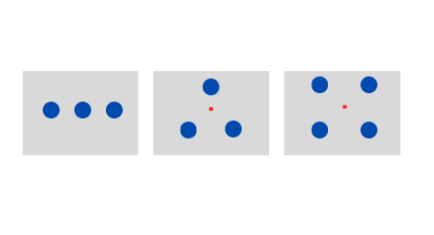
\includegraphics[scale=0.4]{formation}
\caption[formation]{formation}
\end{figure}

\pagebreak
\subsubsection{Shape generation}
The center or leader robot will travel to a specific location in space to initiate the formation of the various shapes. From there, he will inform the other robots of the intended shape to be produced by indicating to them their target position relative to his position at a specific distance and angle.


\subsubsection{Shape formation Algorithm}


\begin{algorithm}[H]
\caption{Shape Formation Algorithm}
\label{alg:ddpg}
\begin{algorithmic}[1]

\State Initialize $n=N$ number of robots.
\State Initialize $c=0$ goal counter.
\State Assign each robot an id starting from $id=1...N$

\State Set the central robot with $id=1$.
\State The central robot moves to a random location and fixes itself there.

\State The central robot broadcasts a message containing his position and the desired shape by generating a set of coordinates that each robot must reach.
\While{$c!=N$}
\For{robot in robots}
\State Take an action.
\State Inform the central robot with his current positions every $t seconds$.
\If{target position reached} 
    \State Stop the robot and inform the central robot.
    \State $c++$ 

\EndIf 

\EndFor

\EndWhile

\end{algorithmic}
\end{algorithm}

\subsubsection{Explanation}



The first robot will choose and occupy a random location. Then, he generates a shape by using the distance and the angle from his current location. After that, he broadcast a message to other robots that contained his position and the target locations. Once the message has been received by the robots, each one of them will attempt to attain the desired goal autonomously by avoiding collisions. And when they have accomplished their mission, they will notify the central robot. Once every robot is in position, the center robot will assess the state of the formation and, if the shape is correctly created, proclaim the task successful.




\subsection{State Representation}

\subsubsection{Introduction}
The state must be carefully planned in order to produce the right shape since how it is shown will have a direct influence on how well our robot performs in attaining its objectives.


\subsubsection{State Representation}
Our neural networks will receive information about the robots' current states as inputs, and using this information, we can determine the rewards that the robots will receive for acting in the environment.
In our implementation, we have six types of state information: the minimum detected object distance and its angle for collision avoidance; the distance to goal; the angle to goal; the angular velocity; and the linear velocity.



\begin{itemize}
\item \textbf{The distance to goal}: 
The first component in our state representation is the distance to the goal, which will be calculated using the Euclidean distance between the robot and the goal.

\[ D(P,G)=\sqrt{(Py-Gy)^2+(Px-Gx)^2}  \] 

Where P and G are the current homogeneous coordinates of the robot and the target goal respectively.

\item \textbf{The angle to goal}: 
The second component is the angle to the goal. And to find it, we need to calculate the difference between the robot's yaw, which is its orientation around its vertical axis, and the angle between the goal and the robot's positions.


\[ \theta(P,G)=yaw-arctan(P/G)  \] 

 \begin{figure}[h]  
\centering
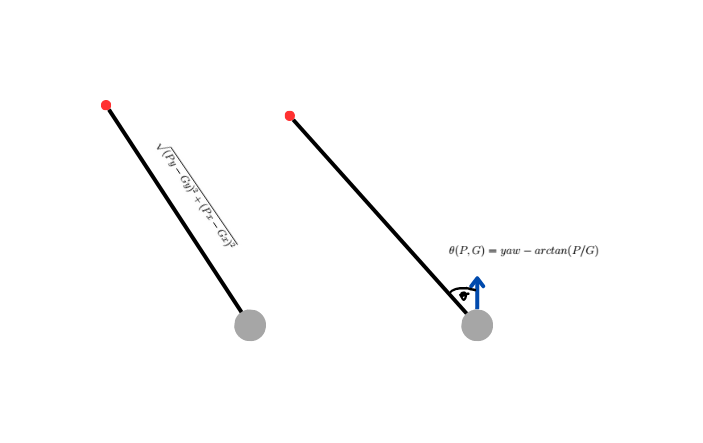
\includegraphics[scale=0.8]{equations}
\caption[equations]{equations}
\end{figure}


\item \textbf{The lds  mesurments}: 
In order to detect other robots and avoid collisions, we use an LDS, which gives us an array of elements where each value is the minimum distance detected and each index is the angle of detection.
The original LDS take 360-degree measurements all around the robot, with a maximum length of 3.5 meters. But in our problem, we don't need such precision, as we have determined that just 50 samples are enough because there are no thin or small objects that require such precision. In addition, we also take just 20 of them, which will cover the front of the robot.

We also added the angle of detection as information to the state, as this helps the robot avoid collisions more effectively.

 \begin{figure}[h]  
\centering
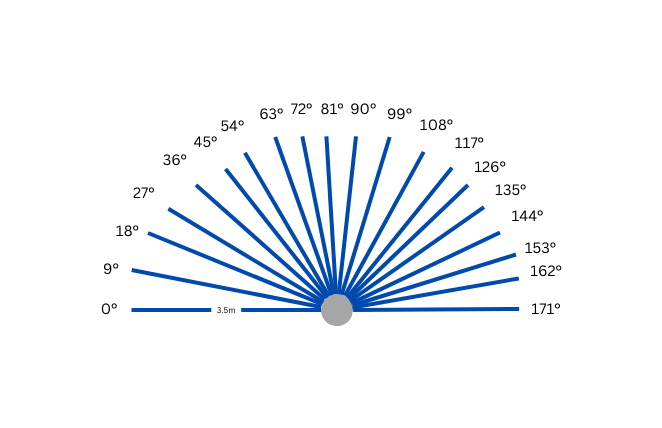
\includegraphics[scale=0.85]{lds3}
\caption[lds mesurement]{lds mesurements}
\end{figure}






\item \textbf{The angular velocity}: 
It is the angular or rotational movement of the robot, and it's between 
$ -\Pi $ and $\Pi$.

\item \textbf{The linear veloctiy}: 
It is the linear speed of the robot. and we have set it between 0.2 and 0.5 m/s.

\end{itemize}



So, our final state representation is an array of:

state=[distance,angle,angular velocity,linear velocity,lds angle,
min lds distance,lidar mesurments]

where lds is a 20 element array.

\subsection{Reward Function Design}

The reward function design is a critical part of any RL system. A well-designed reward function will give the robot more feedback when acting in the environment, thus making the task more 
The reward function was designed to encourage and reward the robot more when he approaches the goal target and penalize him when he collides with the wall or other robots.
The design of the function is based on the state. We have used the distance, the angle, and the LDS to form the final function.
We have divided the function into three parts: The first part is the distance reward. We will give the robot more reward when he achieves the target goal and less when he doesn't.
   
\setcounter{equation}{0}

       \begin{equation} \label{dist_r}
     R_{D}=-D_{goal}
   \end{equation}
 Where $D_{goal}$ is the changing distance between the robot and the target goal, and the second part is the angle of the robot to the goal. formally:


     \begin{equation} \label{angle_r}
     R_{\theta}=-\theta_{goal}
   \end{equation}
 
 where $\theta_{goal}$  ranges  between $-\pi$  and $\pi$.
 
And to avoid collisions between the robots and the wall, we have set two values. The first one is set when the robot approaches the object, which can lead to a collision. And the second one is when it actually collides with it.


\begin{equation}  \label{obs_r}
  R_{c}=\begin{cases}
    -10, & \text{if $mdd< 0.8m$}.\\
    -500 , & \text{ if $mdd <0.20m$ (a crash )}.\\
    0 & \text{ else}.
  \end{cases}
\end{equation}
where $mdd$ stands for the minimum detected distance.\linebreak
Finally, we can add \ref{dist_r}, \ref{angle_r} and \ref{obs_r} to form the finale reward function: 

 
    \begin{equation} \label{final_r}
     R=R_{D}+R_{\theta}+R{c}
   \end{equation}






\subsection{Shape Formation And Deep Reinforcement Learning}
\subsubsection{Introduction}




Each robot will have its own neural network, which will guide him towards the goal positions by avoiding collisions with other robots.
As mentioned earlier, we have used the DDPG algorithm, where each robot will have two neural networks: the critic and the actor.
The actor model will get as input the mentioned state and output two actions: the angle and the velocity.
The robot will learn to move towards the goal by adjusting the angle and will use the velocity to learn how to move faster in certain conditions and slower in others. For example, the velocity will help him with collision avoidance. If he doesn't detect any robots in front of him, he moves faster; otherwise, he slows down.

For the critic, he gets as input both the state and the actions and outputs the q-value, which will be used by the actor to choose the suitable actions to take.
The parameters of both networks will affect the performance of the robots and the speed of convergence. We will describe in detail the parameters that we have chosen to be good for achieving the task.

\subsubsection{The learning flow}
Here, we will describe the learning flow that the robots will go through to learn how to approach their goals.
It starts with the robot being in a given state; he then takes an action, receives sensor data from the sensors like LDS and IMU, and then, based on them, calculates the reward function, and finally, the robot transitions to a new state.
This information (state,action,reward,next state) will be stored in a replay buffer to be sampled from during the training of the models, and once he reaches a certain number of experiences, the training starts.


If all robots reach their goal, the simulation is reset and another formation shape is generated in order to prevent overfitting a certain type of shape.
And if they collide, the simulation is reset, and the robots try again to form the desired shape.
This learning flow will continue until the models converge and the robots form the shapes many times, respectively.
To provide the robots with a notion of what it's like to attain a goal in terms of actions to take and states to be in and to facilitate exploration, we assign relatively basic objectives to be completed in the beginning, and after our robots are familiar with achieving their destinations, we raise the challenge and randomize the target goals.


 \begin{figure}[h]  
\centering
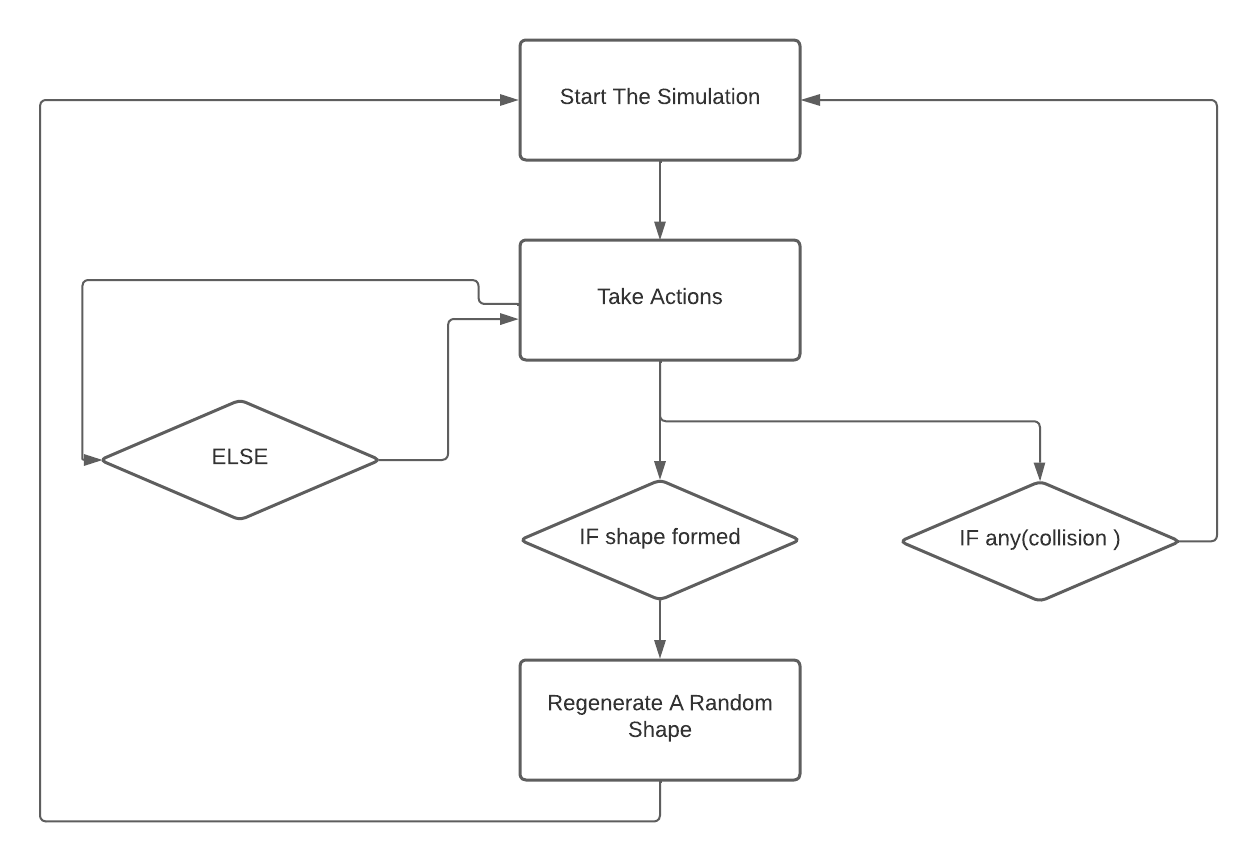
\includegraphics[scale=0.85]{simulation_flow}
\caption[simulation flow]{simulation low}
\end{figure}







 \begin{figure}[h]  
\centering
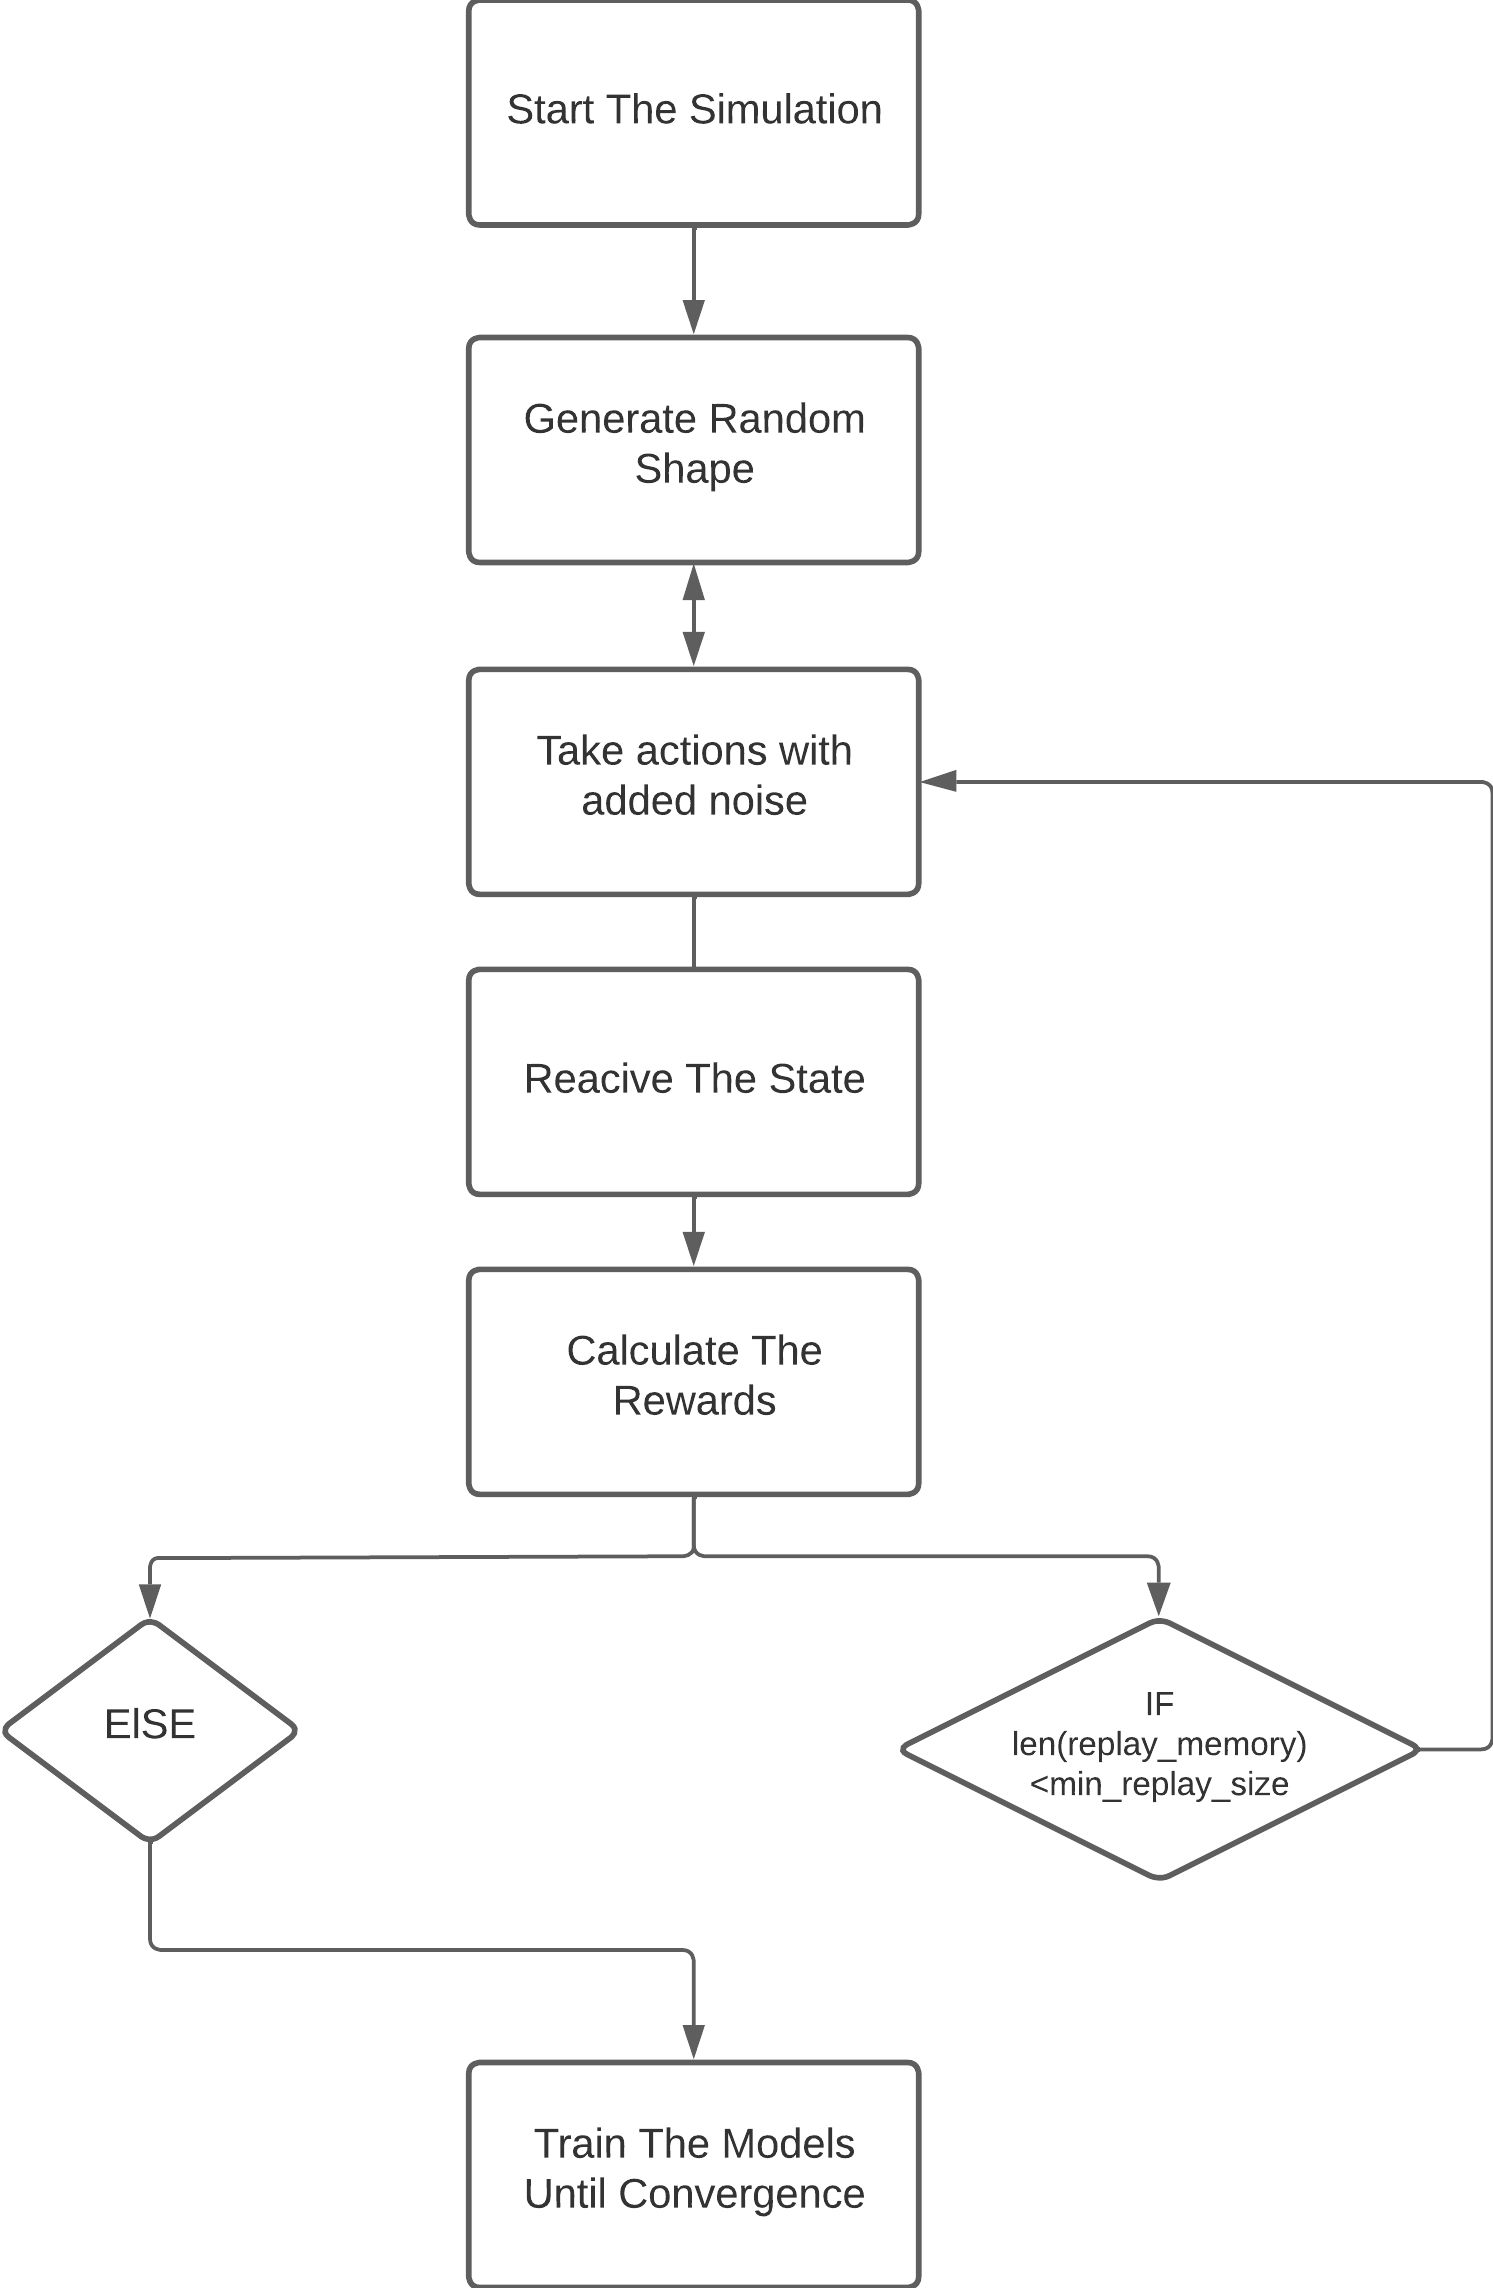
\includegraphics[scale=1.8]{training_workflow3}
\caption[training flow]{training flow}
\end{figure}

\subsection{Conclusion}:
We have presented the problem, it's formulation and our proposed solution in this chapter. Then we explained how the robots' state was represented and how the reward was determined. Finally, we described the learning flow in the simulation.

\afterpage{\clearpage}

\newpage
\pagebreak
\hspace{0pt}
\vfill
\begin{center}
\section{Implementation}
\end{center}
\vfill
\hspace{0pt}

\pagebreak




\subsection{Introduction}
In this section, we will explain how we have implemented the solution, how the neural networks are designed, and what frameworks, tools, and simulators were used to train and test the robot's shape formation.











\subsection{Roboting Operating system}
To implement our work and test it, we used the robot operating system (ROS), which is a collection of open source software and tools that simplifies our work by giving us the necessary tools for controlling the robots, determining their positions and angles, gathering sensor data and preparing it for manipulation, and also giving the robots a way to communicate with one another.
\subsubsection{Ros Basics}
There are five concepts that ROS is built on that will allow us to implement our solution in a simple and modular way.


 

\begin{itemize}
\item \textbf{Nodes}: Ros is made up of nodes, where each node is responsible for a single task like moving the robot, getting sensor data, doing some processing, etc. Nodes can communicate with each other using topics and services.
Each node can subscribe to or publish on one or more topics. He can also contain one or more services that other nodes can request to get one-time information. This approach used by Ros will allow for modularity and more organized and clean code.



\item \textbf{Topics}:Topics are a way for nodes to communicate between themselves. Each node can either subscribe to a topic, thus receiving information from other nodes, or publish to a topic to send information to other nodes.
For example, a node can subscribe to a topic that publishes the position of the robot from another node that is responsible for providing this information.
When defining the topics, we first need to define the exact type of information that they will receive. For instance, we can define topics to accept only strings,  type of information that they will receive. For instance, we can define topics to accept only strings, numbers, or arrays, or we can define our own custom data type..


\item \textbf{Services}:  They are the same as topics, but they differ in that data is received when requested by a client, in contrast to topics where there is a stream of data updated continuously. This can be helpful in situations where the information is needed only once or the update frequency is low.

For example, we can have a service that generates goals or resets the simulation.
As with topics, we must set the data type that the services work with.

\end{itemize}
 

 
 \begin{figure}[h]  
\centering
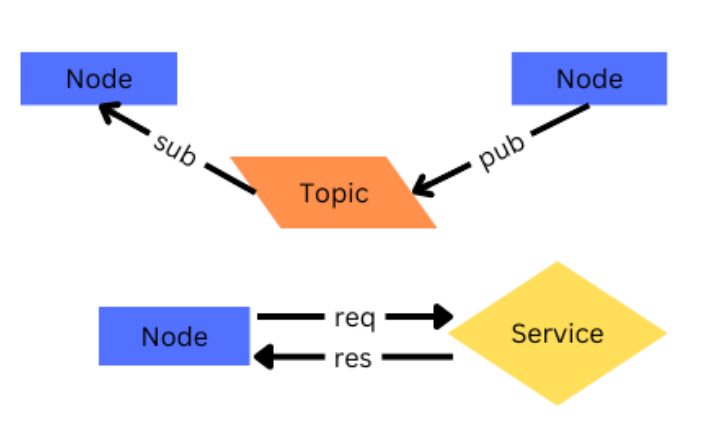
\includegraphics[scale=0.4]{ros}
\caption[Ros]{Ros}
\end{figure}




Ros supports C, C++, or Python as programming languages. In our project, we chose Python. For the operating system, Ros supports mainly Linux systems; support for Windows was added only recently. We have used Ubuntu for the existing support and large ros community.







\subsection{TurtleBot}
We will be using the Turtlebot robot, which was developed by Open Robotics. The same organization is behind Ros and the gazebo simulator.
This robot is used for educational, research, and prototyping purposes, where multiple versions have been developed. In this thesis, we will be using the Turblebot 3-burger version.\cite{turtlebot}

\subsubsection{TurtleBot3 components}
TurtleBot3 is a two-wheeled, small, lightweight robot equipped with a variety of sensors, including a 360-degree laser rangefinder for obstacle avoidance and an IMU for navigation and localization. The robot is powered by a Raspberry Pi single-board computer and is compatible with ROS.
 \begin{figure}[h]  
\centering
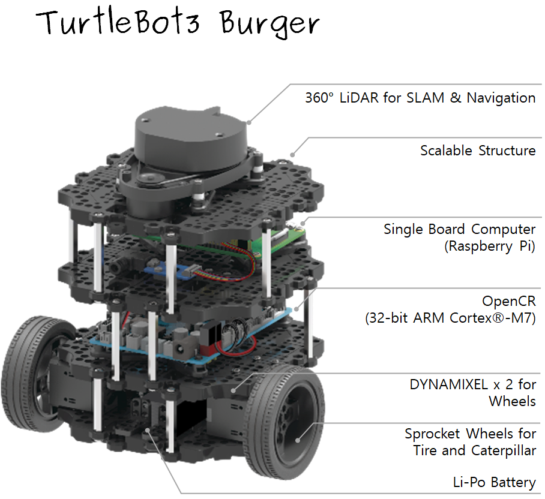
\includegraphics[scale=0.4]{turtlebot3_burger_components.png}
\caption[TurtleBot3]{TurtleBot3 [\textbf{ref}:https://emanual.robotis.com/]]}
\end{figure}

\begin{itemize}
\item \textbf{LDS}:  LDS, which stands for laser distance sensor, which uses lasers to detect the distance between the robot and its surroundings to allow the robot to navigate in the environment and avoid detected obstacles. The LDS used in this project can sense objects in 360 degrees with a maximum length of 3.5 meters. The LDS was one of the data sources used to train our neural networks besides the robots positions. We have used it to detect other robots and avoid collisions during navigation. We have minimized the original 360-degree sample from the LDS as there is no need for such precision in our project.

     
\item \textbf{IMU}: IMU, which stands for Inertial Measurement Unit, is a type of electronic sensor that is used to measure the orientation, position, and velocity of a moving object. The IMU combines information from many sensors, such as accelerometers, gyroscopes, and magnetometers, to give a thorough picture of the movement of the object in three dimensions. The position of the robot is calculated relative to a fixed reference frame, which is either defined by the system designer, like a closed room or factory, or by the robot himself in an outdoor environment.






\end{itemize}

   



\subsection{Simulation}
It's hard, time-consuming, and costly to train the robots in the real world. For that, simulation is used to train the robots, as it allows us to train in a faster, repeatable way and lets us put the robots and the environment in different conditions for faster experimentation.

Robotics simulation programs like Gazebo, Webots, V-REP, MATLAB Robotics System Toolbox, and CoppeliaSim are some of the more well-liked ones. Each one of them has its own features, from programming language support to a fee.
In our project, we used the Gazebo Simulator because it is free, open source, and integrates well with Ros.
Gazebo is an open-source collection of software libraries that have been developed for robotics developers and educators.
It allows you to simulate robotic systems in a virtual environment, providing a safe and cost-effective way to test and refine robot designs before deploying them in the real world. It contains a lot of prebuilt sensors and gives the user the ability to build custom ones. The gazebo is also able to simulate real-world physical phenomena, including physics-based motion, collision detection, and sensor simulation.
  
 \begin{figure}[h]  
\centering
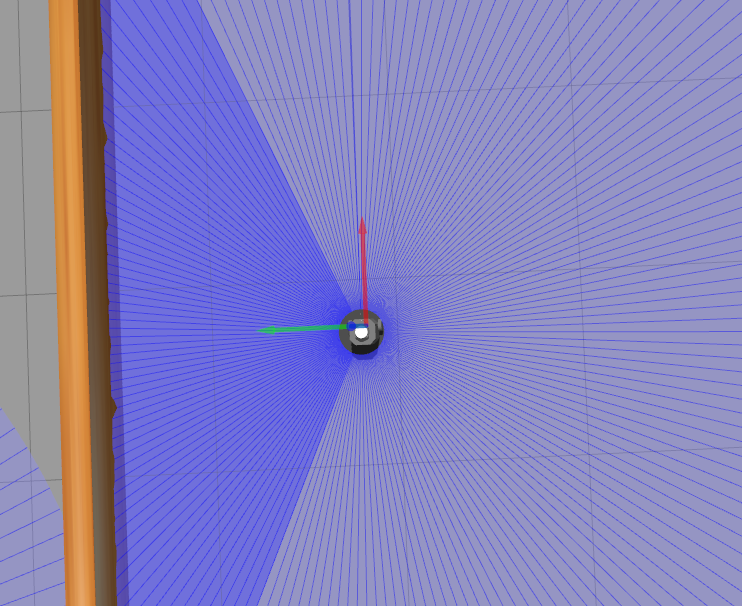
\includegraphics[scale=0.4]{lds.png}
\caption[Lds]{TurbleBot3 Lds}
\end{figure}






 
   











 

\subsection{Ros implemation}
In this section, we will describe how we have implemented our solution in ROS and how we defined the different nodes, topics, and services that make up the system.
The work is divided into two phases. The first is the training and testing phase, and the second is the deployment phase.
In the first phase, we implemented the solution in ROS in a way to facilitate the training process, which will require a lot of modification of code and simulation replay. In this phase, we haven't set up the networking between the robots, as we assume that each robot knows his target position and that we can access the global state.

In the second phase, after the models are trained, we will deploy them in each robot, and each robot will choose its actions based on its model and also communicate with the central robot for coordination.



\subsection{Ros implemation: Training phase}

We have followed the OpenAI Gym implementation of RL problems using the Python programming language.
In the training phase, we have defined two nodes and one Python class for the neural networks.
The first node is the environment node. This node is responsible for getting sensor data, positions, and commands for robots to move in the simulation.
This node has one service, subscribes to two topics, and publishes to one. The first topic he subscribes to is the laser topic, which gets the laser measurements of each robot at every step. The data returned by this topic is an array where each element contains the distance of the detected object, and the index of this element is the angle of detection.

The second topic he subscribes to is the odometry topic, which will get the x and y coordinates of the robots and also their orientation. For sending actions to be executed by the robots, this node will publish to a ROS-defined topic called "cmd vel," which accepts a message that contains the linear and angular velocity of the robot.

The service that this node offers for the main node is a function that will take those actions that the robots should take, get the states, calculate the rewards, and then pass back the response to the main node.


The second node we defined is called the main node. This node is responsible for starting the main training loop, getting actions from the models, passing them to the environment node in order to receive the next states and rewards, then storing these samples in the replay memory, and finally training the models. The loop will continue until the models converge and the shapes are formed. This node will connect to a Python class that contains our models.

This Python class defines the models and the network architecture, contains the replay memory, and describes the training process.





 \begin{figure}[h]  
\centering
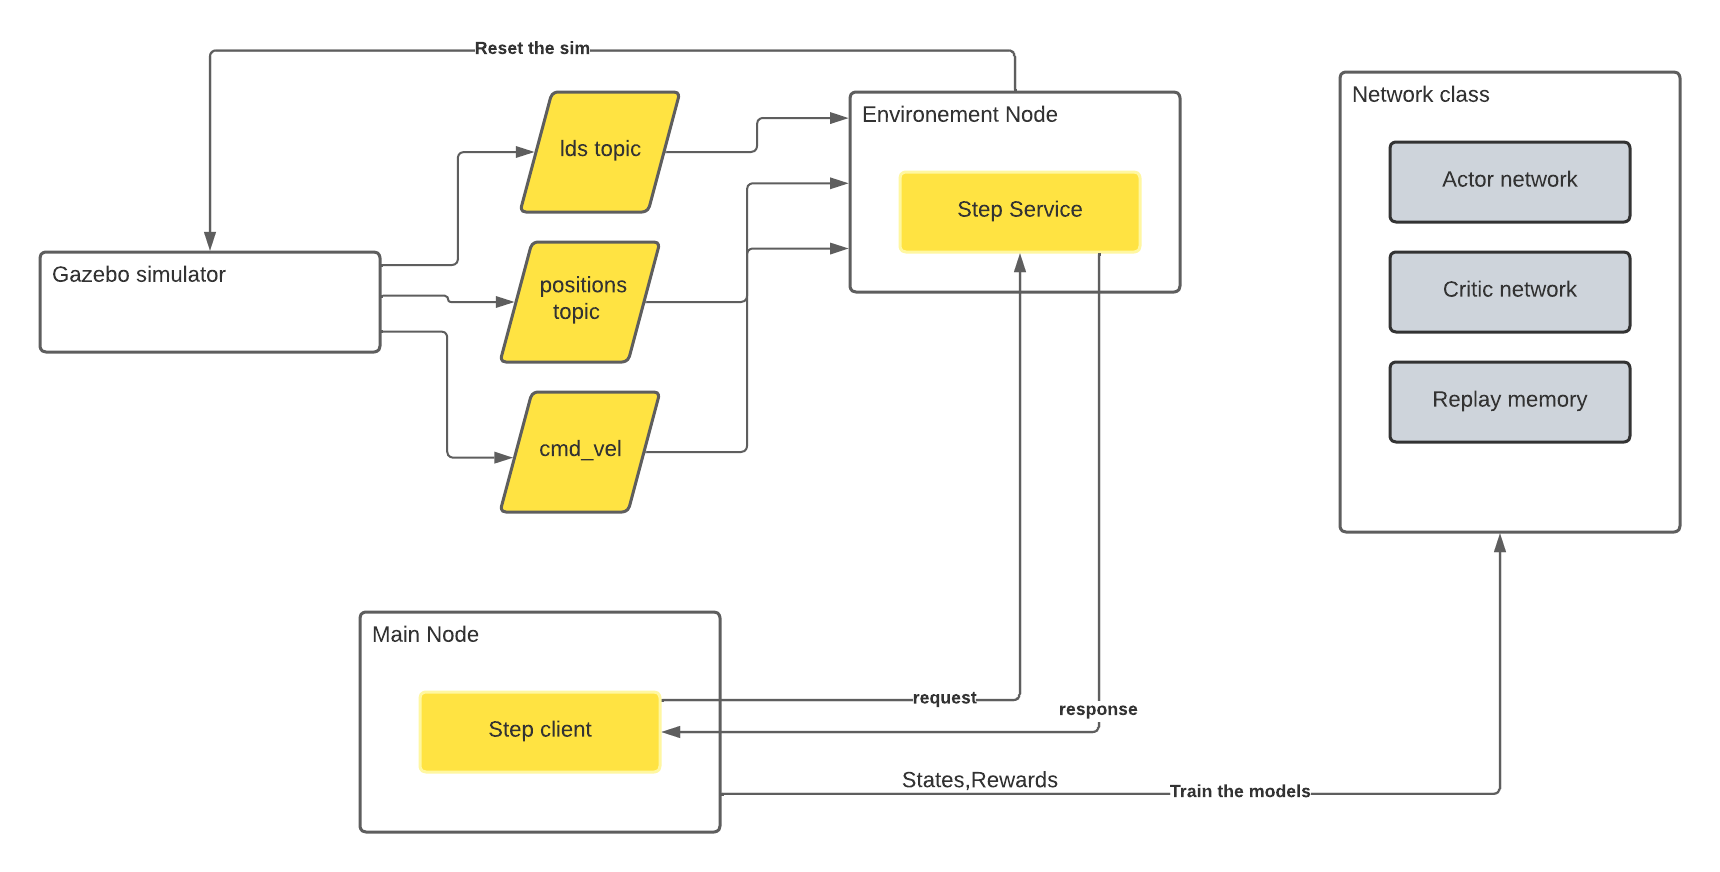
\includegraphics[scale=0.6]{training}
\caption[training phase]{training}
\end{figure}

\pagebreak
\subsection{Ros implemation: Test phase}
In this phase, and after the training of the models is done, we will deploy just the actor models on each robot (no need for the critic as no training is happening) in order to predict actions based on the input state.
We have set up a node for each robot; therefore, communication will take place between these nodes by defining custom topics. Each node will get input states and pass them to the actor model to predict the actions to take.
We have defined one topic called the goals topic, in which the central robot publishes the goal positions and others subscribe to it.  We have also defined a service in the central robot that others will send requests to either inform him about their current position or if they have reached the target goal, in order for the central robot to monitor the state of the formation.
Once all robots are in place, the central robot can then check if the shape is properly formed to finally declare that the task is done by broadcasting a message to other robots in the team.
  



 \begin{figure}[h]  
\centering
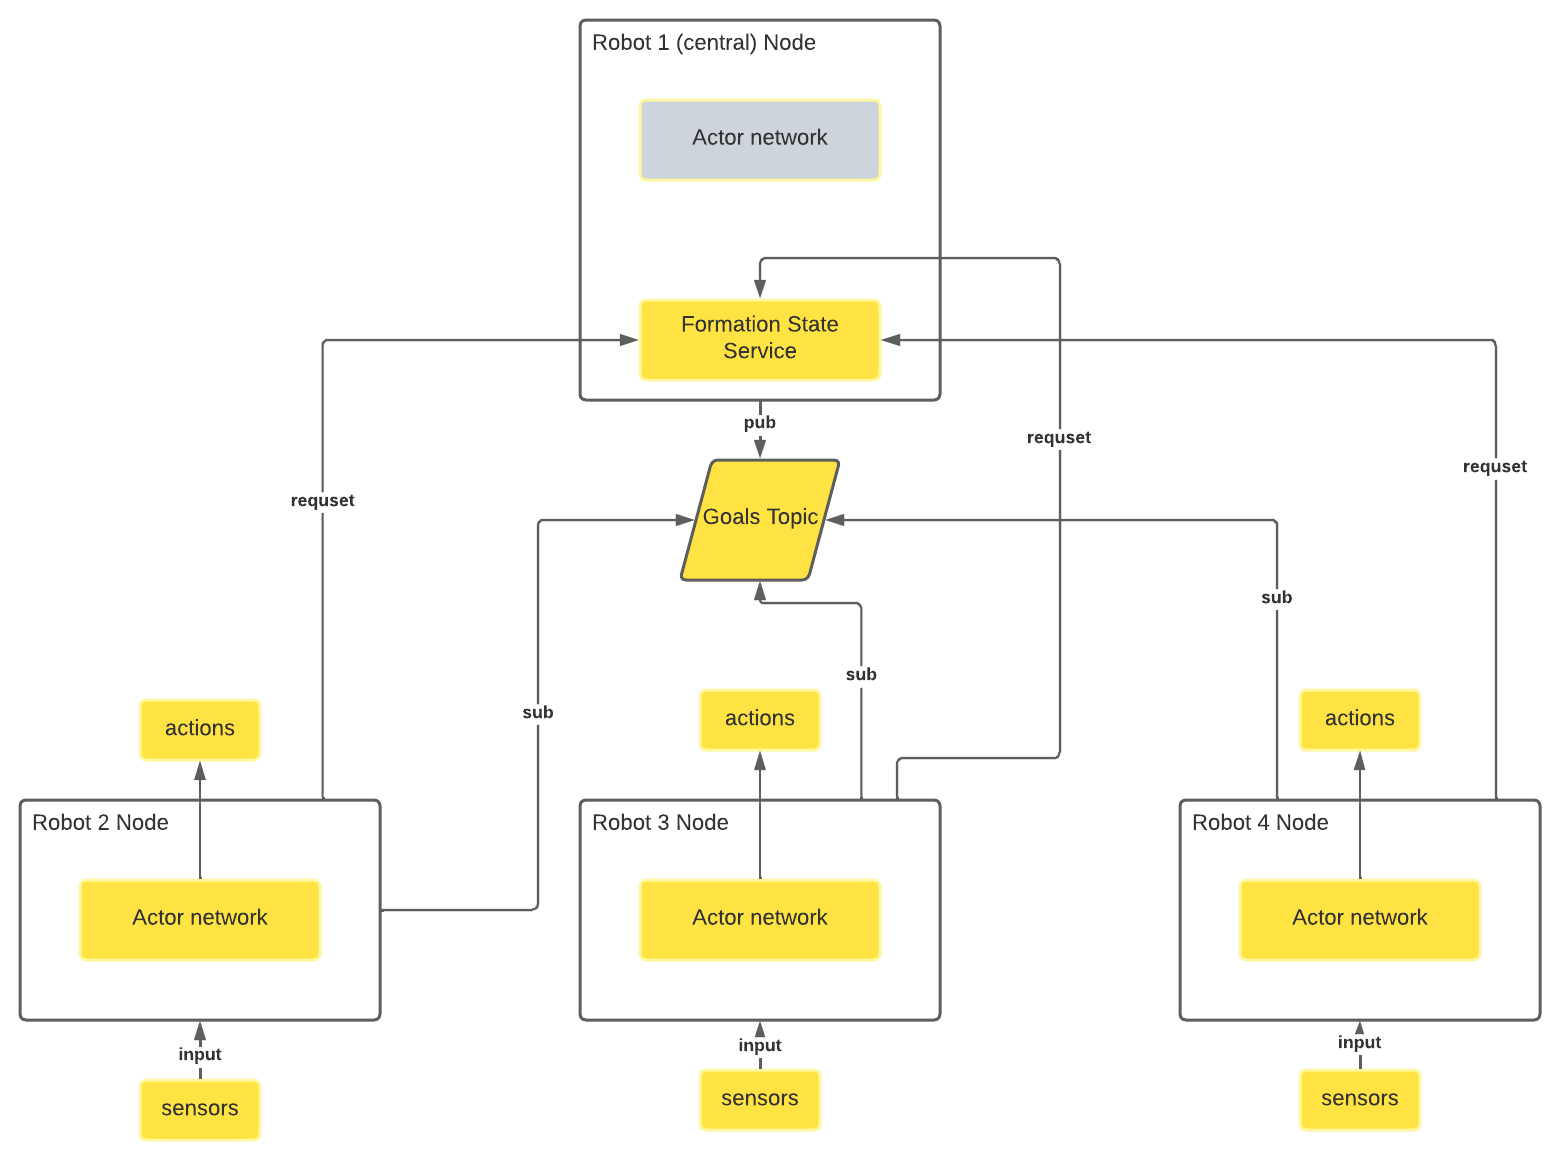
\includegraphics[scale=1.2]{deployment}
\caption[deployment]{deployment}
\end{figure}










 
\newpage




\subsection{Neural network implementation}
Designing the architecture of the neural networks and choosing the right parameters to fit is a crucial part of achieving convergence and better performance. There are a large number of parameters to choose from: hidden layers, number of units, activation functions, weight initialization, regularization, etc. and each one of them has its own role, and there is no clear rule for which one to choose, so trial and error is the way to go. In this section, we will discuss the parameters we choose and explain the reasons behind them.
 
The first thing we have done is normalize the input data to achieve better convergence and stability in our models. We have nominalized our data to be between 0 and 1 for all the inputs:
\newpage
Distance normalization:

  \begin{equation} \label{dist_norm}
     norm_d=distance/dist_{diagonale} 
   \end{equation}
   
where $dist_{diagonale}$ is the diagonal distance of the environment, which is the maximum distance.

Angular velocity and angle to goal normalization:
\begin{equation} \label{angle_norm}
     norm_\theta=angle+\Pi/2\Pi
   \end{equation}

And finnaly the lds mesurements:

 \begin{equation} \label{angle_norm}
     norm_{lds}=lds/3.5 
   \end{equation}
  Where 3.5m is the max length of the lidar sensor.
   
For the actor network, we set four hidden layers where each layer has 400, 300, 128, and 128 units, respectively, with a dropout of 0.3 in the first two layers. Each layer uses the relu activation function and was initialized using Xavier Glorot's except for the output layers, where they were initialized using a uniform distribution. The output layers have two units: one for the angular velocity and one for the linear velocity. They use the Tanh activation function, which gives an output bound between -1 and 1. We chose the angular velocity of the robot to be between $-\Pi $ and $\Pi $ so we multiplied the result of the output layer to get the desired range. The same goes for the linear velocity, we have mapped the range from -1 and 1 to 0.2 and 0.5.

And to enable better exploration, we have added the OuNoise to the output of the actor network when taking actions, which will sample a range of values from a uniform distribution.


We have also used batch normalization layers \cite{ioffe2015batch} which a technique for normalizing the output for each layer that has the effect of stabilizing the training process and making it converge faster, especially if the initial distribution of the input data is varying.

As for the critic, he gets as input both the state and actions and outputs the q-value. Firstly, we pass the states and actions into separate layers with a number of units of 512 and 256, respectively. Then, we concatenate them into one layer and add two other hidden layers with 1024 units, a dropout of 0.2, and a l2 regularization of 0.01.
For loss calculation, we will be using target networks like described in the algorithms and updating them using soft updates with a tau parameter of 0.01
The critic loss, will be between the predicted value of the critic network and y:
 

     \begin{equation} \label{critic_loss}
     closs= loss(critic(state,actions),reward+ \gamma*targetcricic(nextstates,nextactions)*(1-dones).
   \end{equation}
 
where the loss function is the mean squared error.
For the actor, it will be the mean predicted value of the critic network multiplied by, as he is trying to maximize the q-value.

\begin{equation} \label{actor_loss}
     aloss= -mean(critic(states,actions))
   \end{equation}
   
We have used the Adam optimizer for both networks with learning rates of 0.01 and 0.001 for the critic and actor respectively. We set the batch size to 128 and the minimum size of the replay buffer before training start to 5000 samples.


 \begin{figure}[h]  
\centering
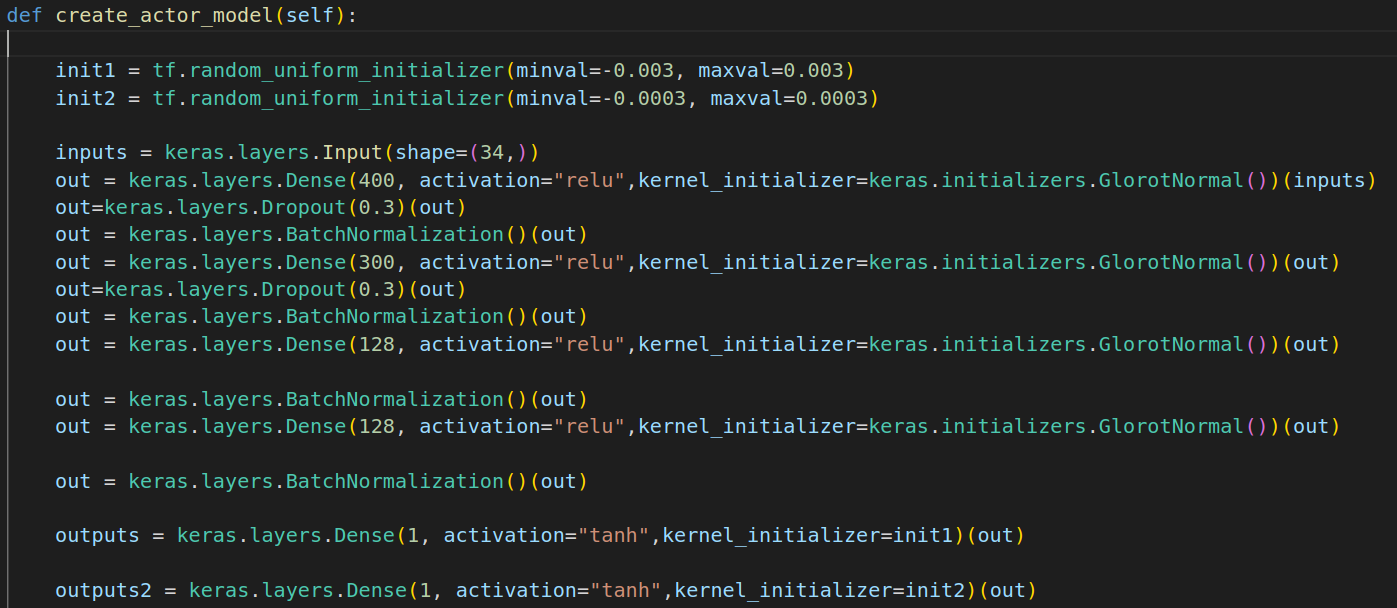
\includegraphics[scale=0.35]{actor_model}
\caption[Actor model]{Actor Model}
\end{figure}





 \begin{figure}[h]  
\centering
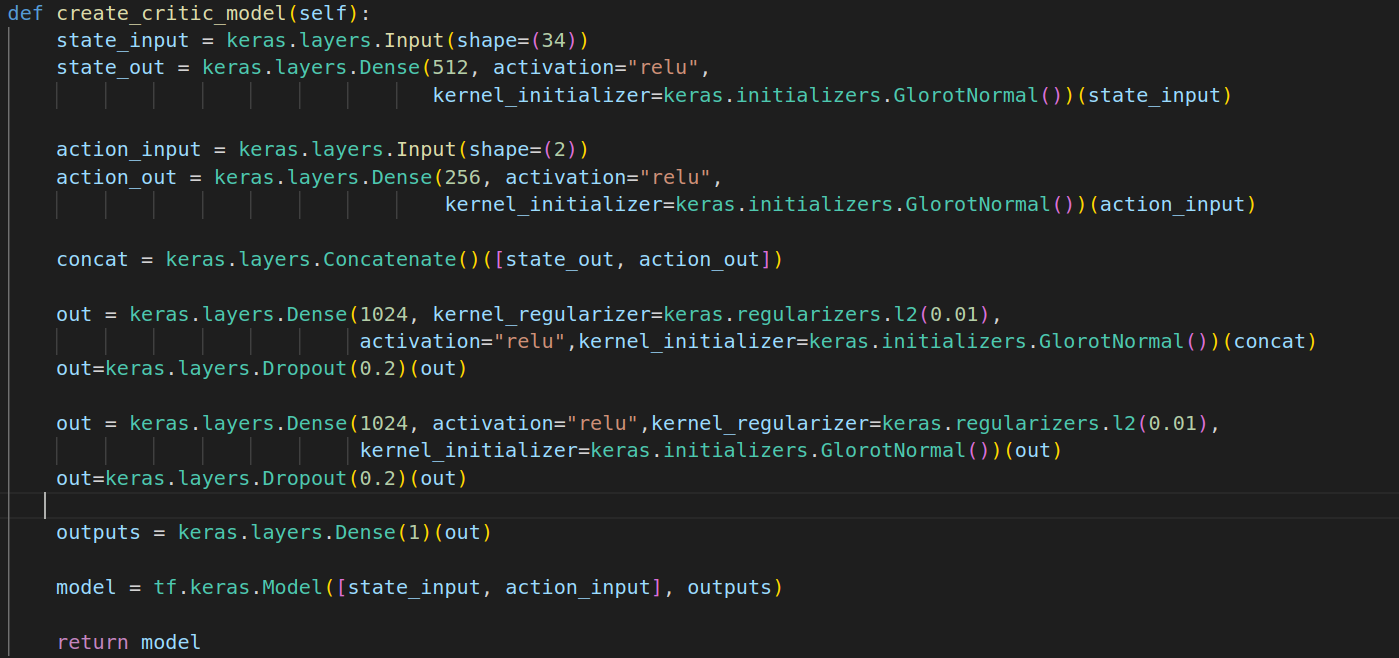
\includegraphics[scale=0.30]{critic_model}
\caption[Critic model]{Critic Model}
\end{figure}





    
 \begin{figure}[h]  
\centering
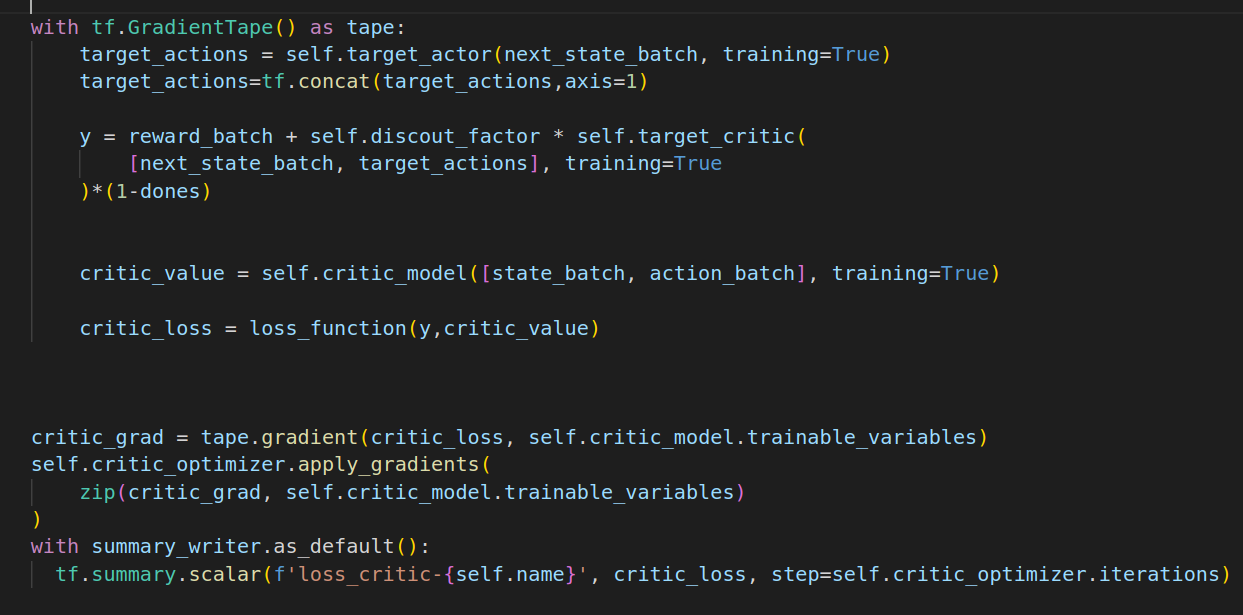
\includegraphics[scale=0.35]{critic_training}
\caption[Critic Training]{Critic Training}
\end{figure}




   
 \begin{figure}[t]  
\centering
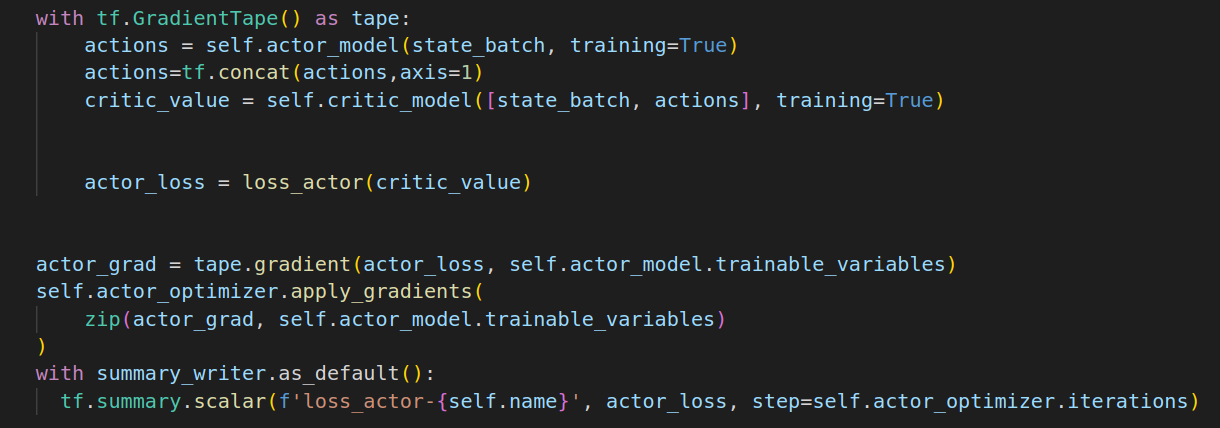
\includegraphics[scale=0.35]{actor_training}
\caption[Actor Training]{Actor Training}
\end{figure}

\subsection{Conclusion}:
In this chapter, we have described how we have implemented our solution in the Ros operating system and gazebo simulator and how we defined the different nodes, topics, and services in ros. Finally, we discussed the architecture of the neural networks and how we chose the parameters.

\afterpage{\clearpage}





\newpage
\pagebreak
\hspace{0pt}
\vfill
\begin{center}
\section{Result and analysis}
\end{center}
\vfill
\hspace{0pt}

\pagebreak

\subsection{Introdution}
\begin{figure}[h]  
\begin{center}
\scalebox{0.3}[0.3]{
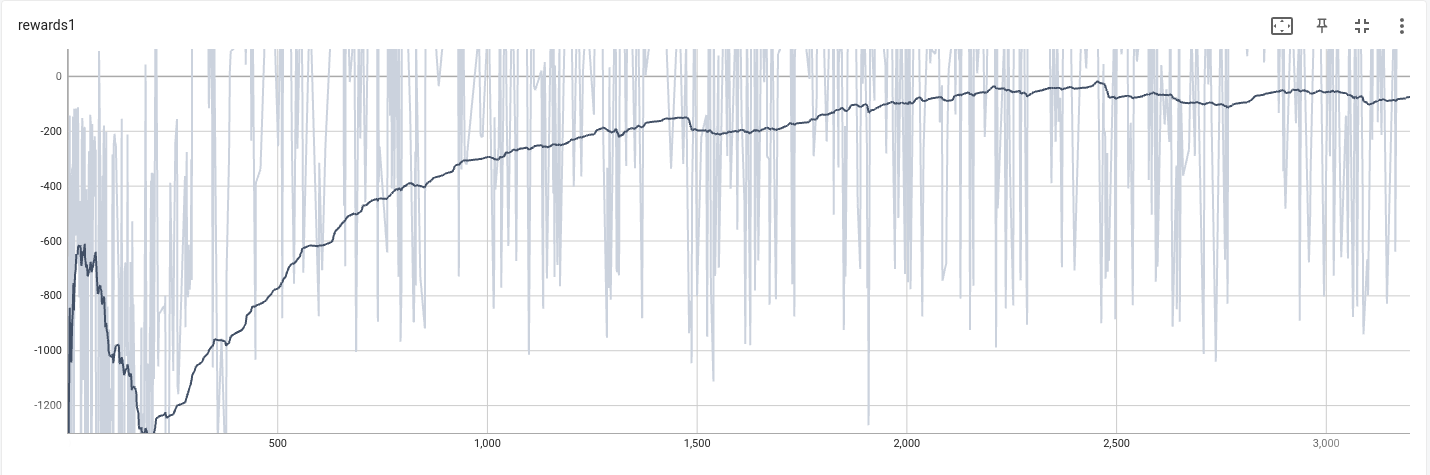
\includegraphics{robot1}
}

\caption[robot1]{robot1}

\end{center}

\end{figure}
\begin{figure}[h]  
\begin{center}
\scalebox{0.3}[0.3]{
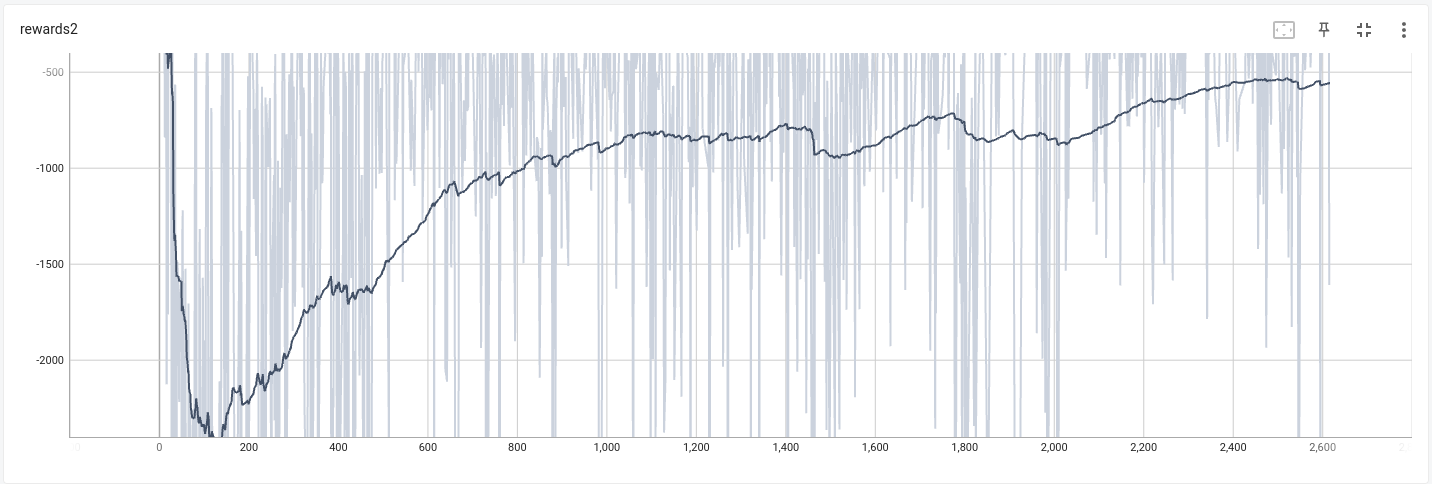
\includegraphics{robot2}
}

\caption[robot2]{robot2}

\end{center}

\end{figure}




\begin{figure}[h]  
\begin{center}
\scalebox{0.3}[0.3]{
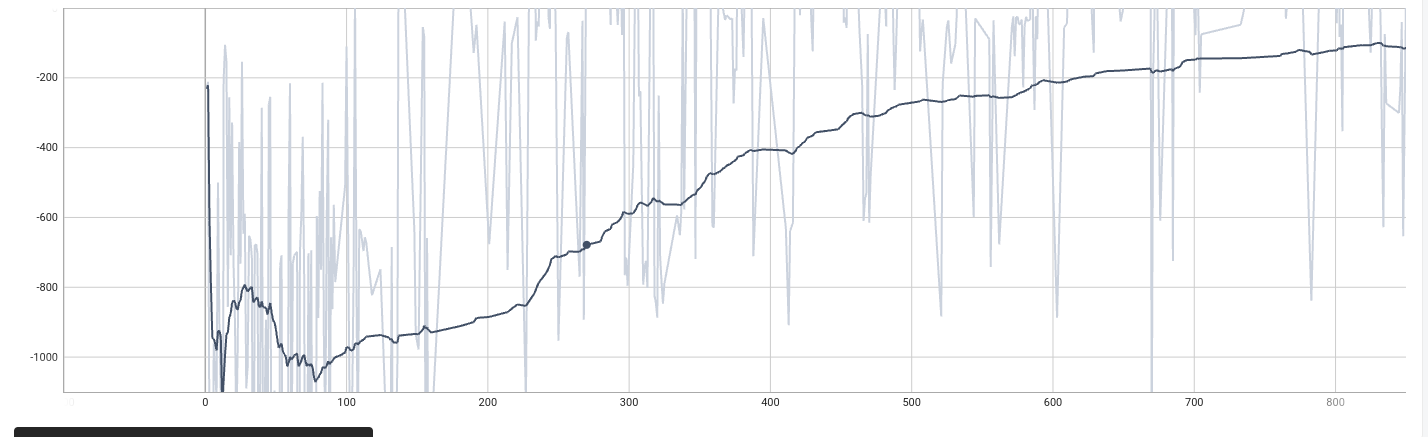
\includegraphics{robot3}
}
\end{center}
\caption[robot3]{robot3}


\end{figure}
In this last section, we will describe the results that we got from our experiment. The training took place between three robots. And to help the robots gradually learn to make the shapes, a range of shapes was created, ranging from easy to difficult.

The training took about 9 hours to finish, and below is the total return of the three robots during the end-to-end training phase.
From the graph, in the first few episodes, the robots gained some rewards easily; this is because the shapes were easy to form. After that, the returns drop quickly when the training starts.

After that, and between episodes 200 and 1500, we can notice that the robots start gaining rewards rapidly, the shapes form frequently, and the collision number decreases.
Finally, from episodes 1500 to 3100, the graph starts to be stable, but the robots still gain some rewards until it converges.
We can also notice that there are some minor differences between the three graphs, as each robot had his own experiences and gained his own rewards separately from the others.

We have deployed our trained models on a team of 4, 5, and 6 robots, where the experiences of the three trained robots were transferred to them.
And to test our solution, we have generated a set of shapes different from those used in the training phase, and below is a table summarizing the total number of shapes being formed without any collision:\\


 
\begin{tabularx}{1.0\textwidth} { 
  | >{\raggedright\arraybackslash}X 
  | >{\centering\arraybackslash}X 
  | >{\raggedleft\arraybackslash}X | }
 \hline
 Number of robots & Total number of shapes & Shapes formed without collision \\
 \hline
 4  & 126  & 95\%  \\
 \hline
 5  & 126  & 88\%  \\
 \hline
 6  & 84  & 82\%  \\
 

\end{tabularx}
\\

The shapes were formed with an accuracy of 92\% for a team of robots with 4 or 5 numbers, but as we increased the number to 6, the accuracy dropped to about 82\%.
Most of the collisions happen when multiple robots meet each other in a small area, where it is difficult for them to avoid complex scenarios. This also happens when the distance between the shape's edges is small.
And most of the collision happened between just two robots; this means that the other ones reached their positions successfully. We have also noticed that the robots avoid collisions perfectly when they are static. This means that if we have a relatively large number of robots, we can command a number of them to reach their destination first, then, with a small delay, tell the others to follow, as this also shows a good result.
Another observation that is related to the last point is that the robot's starting position matters, as some starting positions show good results, especially if not all robots start at the same distance from the goal. \newpage The last observation is that robots tend to form the shape more accurately if the distance between the shape edges is larger.
 

\subsection{Limitations And Future Work}:

Our solution works fine when the number of robots is 3, 4, or 5. but as long as the numbers increase, the performances also decrease. And this can be solved using different types of algorithms that operate on a large number of agents. One of them is the MADDPG algorithm, which is a variant of the ddpg algorithm where the agents not only observe their local state but also the global state during the training, which helps the robot take actions not only based on their local state but also the global state.










\begin{figure}
\centering
\begin{subfigure}{.5\textwidth}
  \centering
  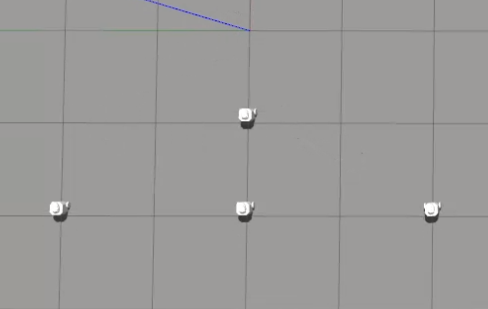
\includegraphics[width=.9\linewidth]{shape1}
  \caption{shape1}
  \label{fig:sub1}
\end{subfigure}%
\begin{subfigure}{.5\textwidth}
  \centering
  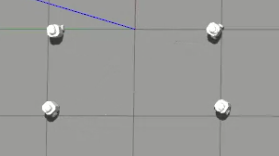
\includegraphics[width=.9\linewidth]{shape2}
  \caption{shape2}
  \label{fig:sub2}
\end{subfigure}
\caption{shapes1}
\label{fig:test}



\end{figure}



\begin{figure}
\centering
\begin{subfigure}{.5\textwidth}
  \centering
  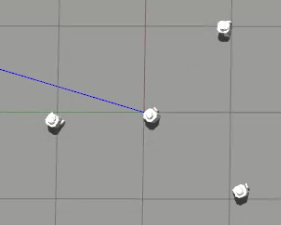
\includegraphics[width=.9\linewidth]{shape3}
  \caption{shape3}
  \label{fig:sub1}
\end{subfigure}%
\begin{subfigure}{.5\textwidth}
  \centering
  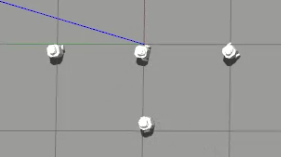
\includegraphics[width=.9\linewidth]{shape4}
  \caption{shape4}
  \label{fig:sub2}
\end{subfigure}
\caption{shapes2}
\label{fig:test}



\end{figure}




\begin{figure}
\centering
\begin{subfigure}{.5\textwidth}
  \centering
  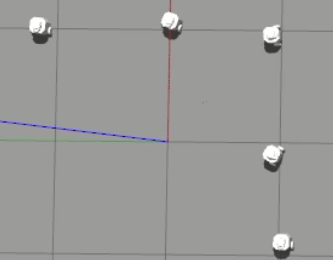
\includegraphics[width=.9\linewidth]{shape5}
  \caption{shape5}
  \label{fig:sub1}
\end{subfigure}%
\begin{subfigure}{.5\textwidth}
  \centering
  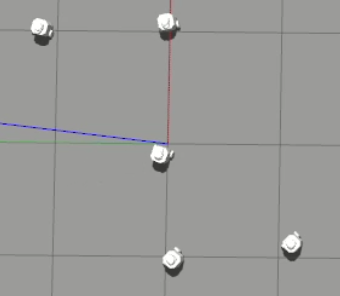
\includegraphics[width=.9\linewidth]{shape6}
  \caption{shape6}
  \label{fig:sub2}
\end{subfigure}
\caption{shapes3}
\label{fig:test}





\end{figure}



\begin{figure}
\centering
\begin{subfigure}{.5\textwidth}
  \centering
  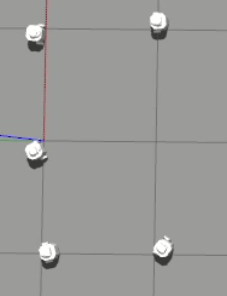
\includegraphics[width=.8\linewidth]{shape7}
  \caption{shape7}
  \label{fig:sub1}
\end{subfigure}%
\begin{subfigure}{.5\textwidth}
  \centering
  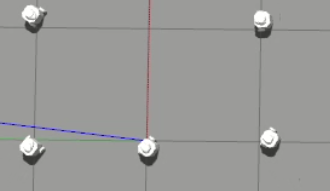
\includegraphics[width=.8\linewidth]{shape8}
  \caption{shape8}
  \label{fig:sub2}
\end{subfigure}
\caption{shapes4}
\label{fig:test}



\end{figure}





\begin{figure}
\centering
\begin{subfigure}{.5\textwidth}
  \centering
  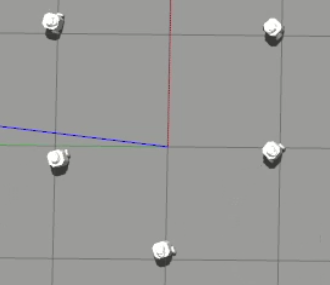
\includegraphics[width=.8\linewidth]{shape9}
  \caption{shape9}
  \label{fig:sub1}
\end{subfigure}%
\begin{subfigure}{.5\textwidth}
  \centering
  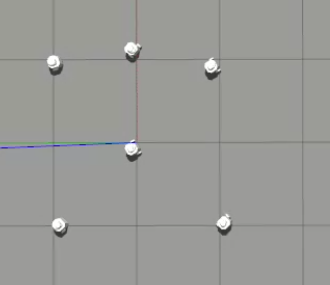
\includegraphics[width=.8\linewidth]{shape10}
  \caption{shape10}
  \label{fig:sub2}
\end{subfigure}
\caption{shapes5}
\label{fig:test}



\end{figure}






\begin{figure}
\centering
\begin{subfigure}{.5\textwidth}
  \centering
  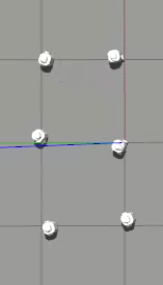
\includegraphics[width=.6\linewidth]{shape11}
  \caption{shape11}
  \label{fig:sub1}
\end{subfigure}%



\end{figure}



\afterpage{\clearpage}
 \newpage
\pagebreak
\hspace{0pt}
\vfill
\begin{center}
\section{Conclusion}
\end{center}
\vfill
\hspace{0pt}

\pagebreak




Swarm robotics is a fast-expanding field that includes coordinating sizable groups of robots to cooperate in order to achieve a common objective. These robots communicate and work together to accomplish tasks that are challenging or perhaps impossible for a single robot to achieve. Swarm robotics is evolving as a result of increased research and development efforts by academics and industry professionals from all over the world, who are continually enhancing the functionality and effectiveness of these systems.



One of the tasks or problems that swarm robots need to solve is pattern formation. Where a group of robots try to form some geometric patterns (lines, circles, rectangles, etc.) in order to do tasks that require such formation, such as object lifting, target encirclement, or military purposes.

There are a lot of algorithms and methods that try to solve this problem. One of them is using reinforcement learning with the help of deep neural networks for their ability to work in highly complex tasks and environments.
In our thesis, we solved the pattern formation problem using a team of robots that try to achieve their target goal with the help of a central robot that will facilitate coordination between the team members and monitor the formation status. Each robot in the team tries to achieve the target goal specified by the central robot autonomously by avoiding obstacles.


We have chosen the DDPG RL Algothim. We have trained three robots to form some geometric shapes, which took about 9 hours to converge.
Then we tested our trained models on a team of 4 and 5 robots, where the learning of the robots was transferred to them, and we got an accuracy of 92\%.
However, the performance of the team decreases as the number of robberies increases, and this can be solved using more suitable algorithms like the MADDPG algorithm, which is a variant of the DDPG.







\newpage
\bibliography{bib}
\bibliographystyle{ieeetr}



\end{document}
